\documentclass[12pt, a4paper]{article}

\usepackage{float}
\usepackage[utf8]{inputenc}
\usepackage{bookmark}
\usepackage{nameref}
\usepackage{graphicx}

\hypersetup{
  colorlinks=true,
  linkcolor=black,
  citecolor=black,
  urlcolor=blue,
}

\usepackage[
  backend=bibtex,
  sortcites=true,
  sorting=none,
  abbreviate=false,
  isbn=false,
  url=false,
  style=authoryear,
  doi=false]{biblatex}
% raggedright to fix bibliography url hbox overflow
\appto{\bibsetup}{\raggedright}
\addbibresource{bibliography.bib}

\graphicspath { {images/} }

\title{A Rusty HTTP Server Library}
\author{Max Cripps}
\date{\today}


\begin{document}

\maketitle \newpage

\tableofcontents \newpage

\section{Aims and Objectives}

In order to develop this project I will need to investigate several RFCs that define the standards
for the HTTP 1.1 protocol. As most HTTP servers are multithreaded, I will also need to investigate
multithreaded implementations that I can use when using Rust. 

The aim of this project is to develop a Rust library that can be used to create an RFC compliant
HTTP application server. The library will contain modular public interfaces so that users of the
library can build an HTTP server, this library will also
have a high level interface for creating an HTTP server application that requires minimal code. I will
be creating multiple example projects to demonstrate using the library and to prove it works as intended,
see \emph{\nameref{sec:deliverables}} for more.

The library will not be \emph{"fully featured"} as providing this in the time frame would not be
possible. A production ready library would require more time in order to fully comply with the RFCs
and to support HTTP2.0 and HTTP3.0, it would also require extensive benchmarking and testing both in
logic and vulnerabilities. This scope restriction in mind, meant that it was important to break the
requirements down and prioritise them in order to provide accurate estimates of what could be achieved.

\section{Requirements} \label{sec:requirements}

Most of the requirements are derived from RFCs that define the HTTP 1.1 protocol and RFCs in which
those depend on. The main RFCs that define the HTTP 1.1 protocol are as follows:
\begin{itemize}
  \item RFC7230 \emph{Message Syntax and Routing}
  \item RFC7231 \emph{Semantics and Content}
  \item RFC7232 \emph{Conditional Requests}
  \item RFC7233 \emph{Range Requests}
  \item RFC7234 \emph{Caching}
  \item RFC7235 \emph{Authentication}
\end{itemize}

All the RFCs listed above follow the requirement notation as defined in RFC2119 (\cite{rfc2119}),
this RFC defines keywords and how they should be interpreted in order to be RFC compliant.

The requirements are grouped under subsections using the MoSCoW prioritization (\cite{moscow}) method.

\subsection{Must Requirements}
\begin{itemize}
    \item\label{mreq:rfc-compliance} RFC compliance
    \item\label{mreq:memory-and-panic-safety} Memory and panic safety
    \item\label{mreq:public-interface-documentation} Public interface documentation
    \item\label{mreq:request-parsing} Request parsing
    \item\label{mreq:configurable-request-validation} Configurable request validation
    \item\label{mreq:status-code-based-errors} Status code based error handling
    \item\label{mreq:response-built-from-request} Response built from request
    \item\label{mreq:response-serialization} Response serialization
    \item\label{mreq:tcp-communication} TCP communication
    \item\label{mreq:example-hello-server} "Hello, World!" server (example deliverable)
    \item\label{mreq:example-echo-server} Echo server (example deliverable)
    \item\label{sreq:example-file-server} File server (example deliverable)
\end{itemize}

One of the major over arching requirement is to make sure that this implementation is memory and panic safe, which
means that, as the server is running that it is not leaking memory due to the library implementation
and cannot access invalid memory addresses. Panic \footnote{A panic in rust is equivalent to an
exception in languages like C\#, Java, JavaScript but is more closely related to Java's runtime
exception where they often not handled by the application.} safety is a further guarentee that the implementation
will uphold memory safety even when panics occur. Rust allows for more fine-grained control over
memory management which comes with dangers and benefits, see more in
\emph{\nameref{sec:choosen-approach}}.

I think a library requires good documentation in order to be usable by others, so this became a must
requirement for this project - it benefits me while implementing too as the design is modular, so I
will likely be using my own documentation.

RFC7230 (\cite{rfc7230}) contains the majority of the syntax for the request and response messages
in the HTTP protocol. The syntax notation used in this RFC is the Augmented Backus-Naur Form (ABNF)
notation of RFC5234 (\cite{rfc5234}). Much of the HTTP standard is based around the message syntax
defined in this RFC, therefore parsing and forming messages is a large part of the implementation.

The implementation of the transport layer even effects how requests need to be parsed; The URI
will accept port numbers as the normal transport layer is assumed to be TCP, however, if the
implementation is not TCP then parsing of URIs need to be more restrictive.

RFC7231 (\cite{rfc7231}) defines the all Status Codes that should be supported by both servers and
user-agents. The Status Codes is a three-digit number which explains the result of the request made
by the user-agent. Many of the other RFCs cross-reference this one when stating intended behaviour
of the server in regard to what status code it should return to a user-agent when a given event
occurs, such as when trying to pass a URI that is too long for the server then the server should
return a 414 (URI Too Long). The importance of status codes meant that I wanted to add them as a
major part of the error handling from beginning which is why it is part of the requirements list.

\subsection{Should Requirements}

\begin{itemize}
    \item\label{sreq:server-logging} Server logging
    \item\label{sreq:multithreaded-request-handling} Multithreaded request handling 
    \item\label{sreq:example-sleep-server} Sleep server (example deliverable)
    \item\label{sreq:request-routing} Request routing
    \item\label{mreq:example-list-server} List server (example deliverable)
\end{itemize}

The URI, adapted from RFC3986 (\cite{rfc3986}), defined in RFC7230 is a major part of defining 
the resource target which will help when implementing the request routing provided by the library,
so that specific functions can be called to handle the request based on its resource target and the
method of the request.

\subsection{Could Requirements}

\begin{itemize}
    \item\label{creq:request-body-deserialization} Request body deserialization
    \item\label{creq:request-query-deserialization} Request query deserialization
    \item\label{creq:caching-service} Caching
    \item\label{creq:transport-layer-agnostic} Transport layer agnostic
    \item\label{creq:asynchronous-request-handling} Asynchronous request handling
    \item\label{creq:conditional-requests} Conditional Requests
    \item\label{creq:range-requests} Range Requests
\end{itemize}

RFC7232 (\cite{rfc7232}) and RFC7233\\ (\cite{rfc7233}) define more semantics and capabilities to the
request syntax defined in RFC7230. These two RFCs and their semantics are a lower priority due to the
size and scope of this project, however, the contents of the RFCs were still researched as part of
the planning and requirements refinement as I want to create the project so that these requirements
could be added if more time to implement them before the deadline.

RFC7235 (\cite{rfc7234}) defines the stanards for caching the response of requests, this is a lower
priority as it provides an optimization for servers, proxies and client to cache responses. As part
of this requirement a cache service could also be implemented to expose more high-level features
from the library.

\subsection{Won't Requirements}

\begin{itemize}
    \item\label{wreq:connect-method-support} CONNECT method support
    \item\label{wreq:http2.0-support} HTTP 2.0 support
    \item\label{wreq:authentication} Authentication service
    \item\label{wreq:proxy-or-gateway} Proxy OR Gateway
\end{itemize}

RFC7230 provides details regarding routing of proxy and gateway implementations that
won't be used in this project.

RFC7235 (\cite{rfc7235}) is the RFC defining authentication and other security considerations. As
a developer who is not an expert in application security I felt that Authentication and HTTPS
requirements were a lower priority for this project, however, for a project to be useful in production,
security must be one of the fundamental building blocks especially for an HTTP application. HTTPS and
authentication would also be more difficult to showcase clearly and correctly as HTTPS would require
certification and authentication would require some storage as part of the examples.

\section{Deliverables} \label{sec:deliverables}

\begin{itemize}
    \item Source code 
    \item Documentation
    \item GitHub repository (confirmation of CI)
    \item Server application examples \footnotemark[1]
      \begin{itemize}
          \item "Hello, World!" server
          \item Echo server 
          \item Sleep server 
          \item File server
          \item List server
      \end{itemize}
\end{itemize}

\footnotetext[1]{The examples delivered will depend on the implementation as the examples listed
demonstrate different features of the library and so if they are not implemented then the example
will not be part of the deliverables, this also means more examples might be provided if more
requirements are implemented}

The main deliverable is the source code for the library, which will be provided in a compressed zipped
folder with the public documentation. The source code would also be available on GitHub as a private
repository, where access will be granted to my supervisor and second reader - the repository will
be made public after the deadline so that moderators would have free access to review, if required.
The GitHub repository is also set up for CI using
\href{https://docs.github.com/en/actions/learn-github-actions/understanding-github-actions}{\emph{GitHub Actions}}
which will run all the unit tests and document tests which should help aid moderators that the code
is working as intended.

\subsection{Examples}

The library itself will be quite a bit of code and would be hard to assert that it works, especially
if you aren't used to reading Rust code, therefore, I will also be including examples of application
servers built using the library code so that they can be run and hand tested.

Each example provided will come with a README that explains how to run the example
and the purpose it is trying to convey. It will also provide a sequence of commands that can be
used to test the example as a guide, these will likely be using curl for unix and Invoke-WebRequest
for Windows.

\subsubsection{"Hello, World!" Server}
This example is the simplest proof that the application can receive a GET request and provide the
simple response "Hello, World!". This will help demonstrate that the parsing of the status-line,
TCP connection is working correctly.

\subsubsection{Echo Server}

This example will provide a simple proof that the application server can receive a request and then
provide a response with the same body content. This will help demonstrate that the parsing, TCP
connection and serialization of the response body is working correctly for simple GET requests.

\subsubsection{Sleep Server}

This example will provide two routes; the first which will always take a number of seconds to return
a response and another that will return a response almost immediately. The reason for this example is
to help demonstrate that the server can handle multiple requests at the same time without blocking
the other. The sleeping route will cause a thread blocking action which could be, but not limited to,
a thread sleep - thread in this context doesn't necessarily denote an OS thread as in an asynchronous
runner the thread would be a green thread.

\subsubsection{File Server}

The file server example will provide a static path for file lookup which can be requested using a
GET request. This will demonstrate using the library to query the request in order to get
the path for the request file and returning that file as a response. This will also demonstrate
possible controls for denying a request that tries to access a file outside the static parent
directory.

\subsubsection{List Server}

The list server example will hold an in memory global list which can be updated using the REST
architectural style (\cite{rest}).
This will demonstrate request routing specifically for different methods and somewhat simulates how
a server could be designed to interact with a database. The main purpose is not to address the problems
of shared mutability of global state in this example, but it could be, given enough time to do so as
this would be a problem that would occur in a real server application.

\section{Choosen Approach} \label{sec:choosen-approach}

A general theme in this project is to use software and tools that promote sharing and
co-operation, this was not just for the development but also for planning and analysis of the
planning. I feel this is more akin to the normal procedure in the industry and allows for teams of
multiple people of different roles to work in an efficient and cohesive manner.

\subsection{Language and Development Tools} \label{ssec:language-and-dev-tools}

One of the first choices and ultimately one of the most impactful was, what programming lanugage
would be best suited to this project. I wanted to assure that the library was memory safe and has
good consistent performance. Memory safety is important because a server application is often a
long-running program, so any memory leaks will cause an \emph{out of memory} error. This requirement
for memory safety made me consider managed languages such as Java or Go, however, with managed memory
comes the garbage collector and this can add some hiccups in performance as found by Discord (\cite{discord}).

I first learnt to code with C++ so this was a consideration, but I had not used it since smart pointers
first got introduced, and I have heard many things have changed since then. I had just started trying out Rust
after seeing it become the most loved programming language on StackOverflow for the sixth year running
(\cite{so-most-loved-lang-2021}), and the mix of low level
control with high level concepts and a sprinkle of functional influence had me convinced that Rust
would be a great language to use for this project. Rust also has a concept of \emph{Ownership},
which was inspired from Cyclone (\cite{cyclone}), that enables Rust to make memory safety
guarentees without needing a garbage collector and the best part of this concept is that it is
completely in the control of the developer and not a runtime. Memory safety is also a major concern regarding
security, both Microsoft (\cite{microsoft-memory-safety}) and the Linux community (\cite{linux-memory-safety})
agree that around two-thirds of security vulnerabilities stem from memory-safety issues.

Rust and the tools it provides were another part of the decision, Rust has a dependency management
tool called Cargo, but it does more than this; it provides a high level command line interface for 
building, testing, benchmarking and running Rust code with documentation.

Source control is a must for development and I have used and know Git very well and use it mostly
with the source control hosting site GitHub. In this project I choose to use Git as I only have
experience with this and Team Foundation Server (TFS), the latter being an unpleasent experience of
legacy code trapped in a legacy source control system. I have good experience using GitHub and
find GitHub Actions as an associated CI tool easy to set up and use for projects that don't require
multiple complex environments. 

\subsection{Planning with Jira}

Jira is an agile project management \emph{Software as a Service} (SaaS). I used Jira in order to
plan my project. I used Jira over Trello as I wanted to perform my implementation in
sprints and not use a Kanban-style. I have also used Jira in my placement year, and I am aware that it 
is used by many companies, therefore, learning more about Jira in the process of this 
project will build up another skill (\cite{jira}).

I researched the information provided by Atlassian regarding \emph{Agile project management},
this includes information on epics, stories, and estimation and how Jira helps. This information
helped me decide that I wanted to use Jira for project management and integrate this with GitHub.
I used the Scrum approach in Jira as I wanted to implement the work in sprints so that after each
sprint I could review the work and state of the project with a different perspective
(\cite{jira-agile-info}). 

\subsection{Implementation} \label{ssec:implementation}

I considered many options for how and in what order I'd be implementing this project. I choose
to implement the request parsing first, this is by far the largest and arguably most important part
of the implementation in regard of RFC compliance; as defined in RFC7230 HTTP is an interface designed
through defining the syntax of communication. Then after implementing the request parsing I will
work on the shared models that will be used by both the request and response, so this will include implementing
deserialization and serialization for requests and responses respectively. Then from this module of
work I can create the "core" of the library which includes setting up TCP conncections and providing
configurable contexts that can effect the parsing of requests. 

An alternative implementation approach I considered was to use existing code as dependencies for the
request and response models allowing me to focus on the "core" of the project which would have afforded
me more time to create a more feature rich library and focus on performance tuning in a multithreaded
environment. This was tempting, however, I felt that a big part of the nature of this project is to
research and implement from an RFC which meant that request parsing was an important part of the
project to implement myself.

\section{Plan} \label{sec:plan}

I am using Agile and some DevOps for my planning. All of my requirements have been split down into
a list of user stories within Jira and initially were part of the sprint backlog.

\subsection{Sprint Planning}

I will be conducting sprints with a duration of two weeks, the stories used for the sprints are
based on priority and following the implementation plan as discussed in \textbf{\nameref{ssec:implementation}}
under the \textbf{\nameref{sec:choosen-approach}} section above. I initially wanted to have sprints of 1 week 
duration, however, because this project is only a part of my workload, a week would not provide enough
time to complete some user stories that reasonably should be completed in a single sprint. The
two-week duration is also beneficial as this coincides with a meeting with my supervisor, so this could
allow for both of us to review some analysis of the completed sprint.

The number of user stories in each sprint is based on story point estimation, I found this made it
easier to estimate single user stories. Sprints created from story point accumulation, I felt would
be easier to adjust after sprint analysis of the burndown charts and velocity report and the number
of story points for each sprint could be adjusted. The user stories themselves are also easier to
change and adapt when using story points and I feel that as I work on the project more that I will
be updating the story points to more accurately represent the complexity of the work.

The user stories are child issues for epics, which are large bodies of work that are delivered over
a period of multiple sprints, this makes it easier in Jira to group user stories based on their epics
respectively. The sprints designed are generally working towards completing a specific epic, however,
due to the scope of the project some work in the epic is a lower priority then work in another
epic and so work on one epic is suspended in order to focus on Must and Should priority stories in 
other epics. This priority based planning of sprints is an attempt to avoid the scenario where only
a certain part of the project is complete but cannot demonstrate any functionality because the
"glue" code hasn't been implemented yet.

Jira provides a roadmap widget [\ref{fig:jira-roadmap}], which is their equivalent to a
simple Gantt chart. I used this as a replacement for a Gantt chart as it stays in sync with Jira and
using something like Jira meets my \textbf{\nameref{sec:choosen-approach}} as discussed in the initial
paragraph of that section.

\begin{figure}[H]
  \centering 
  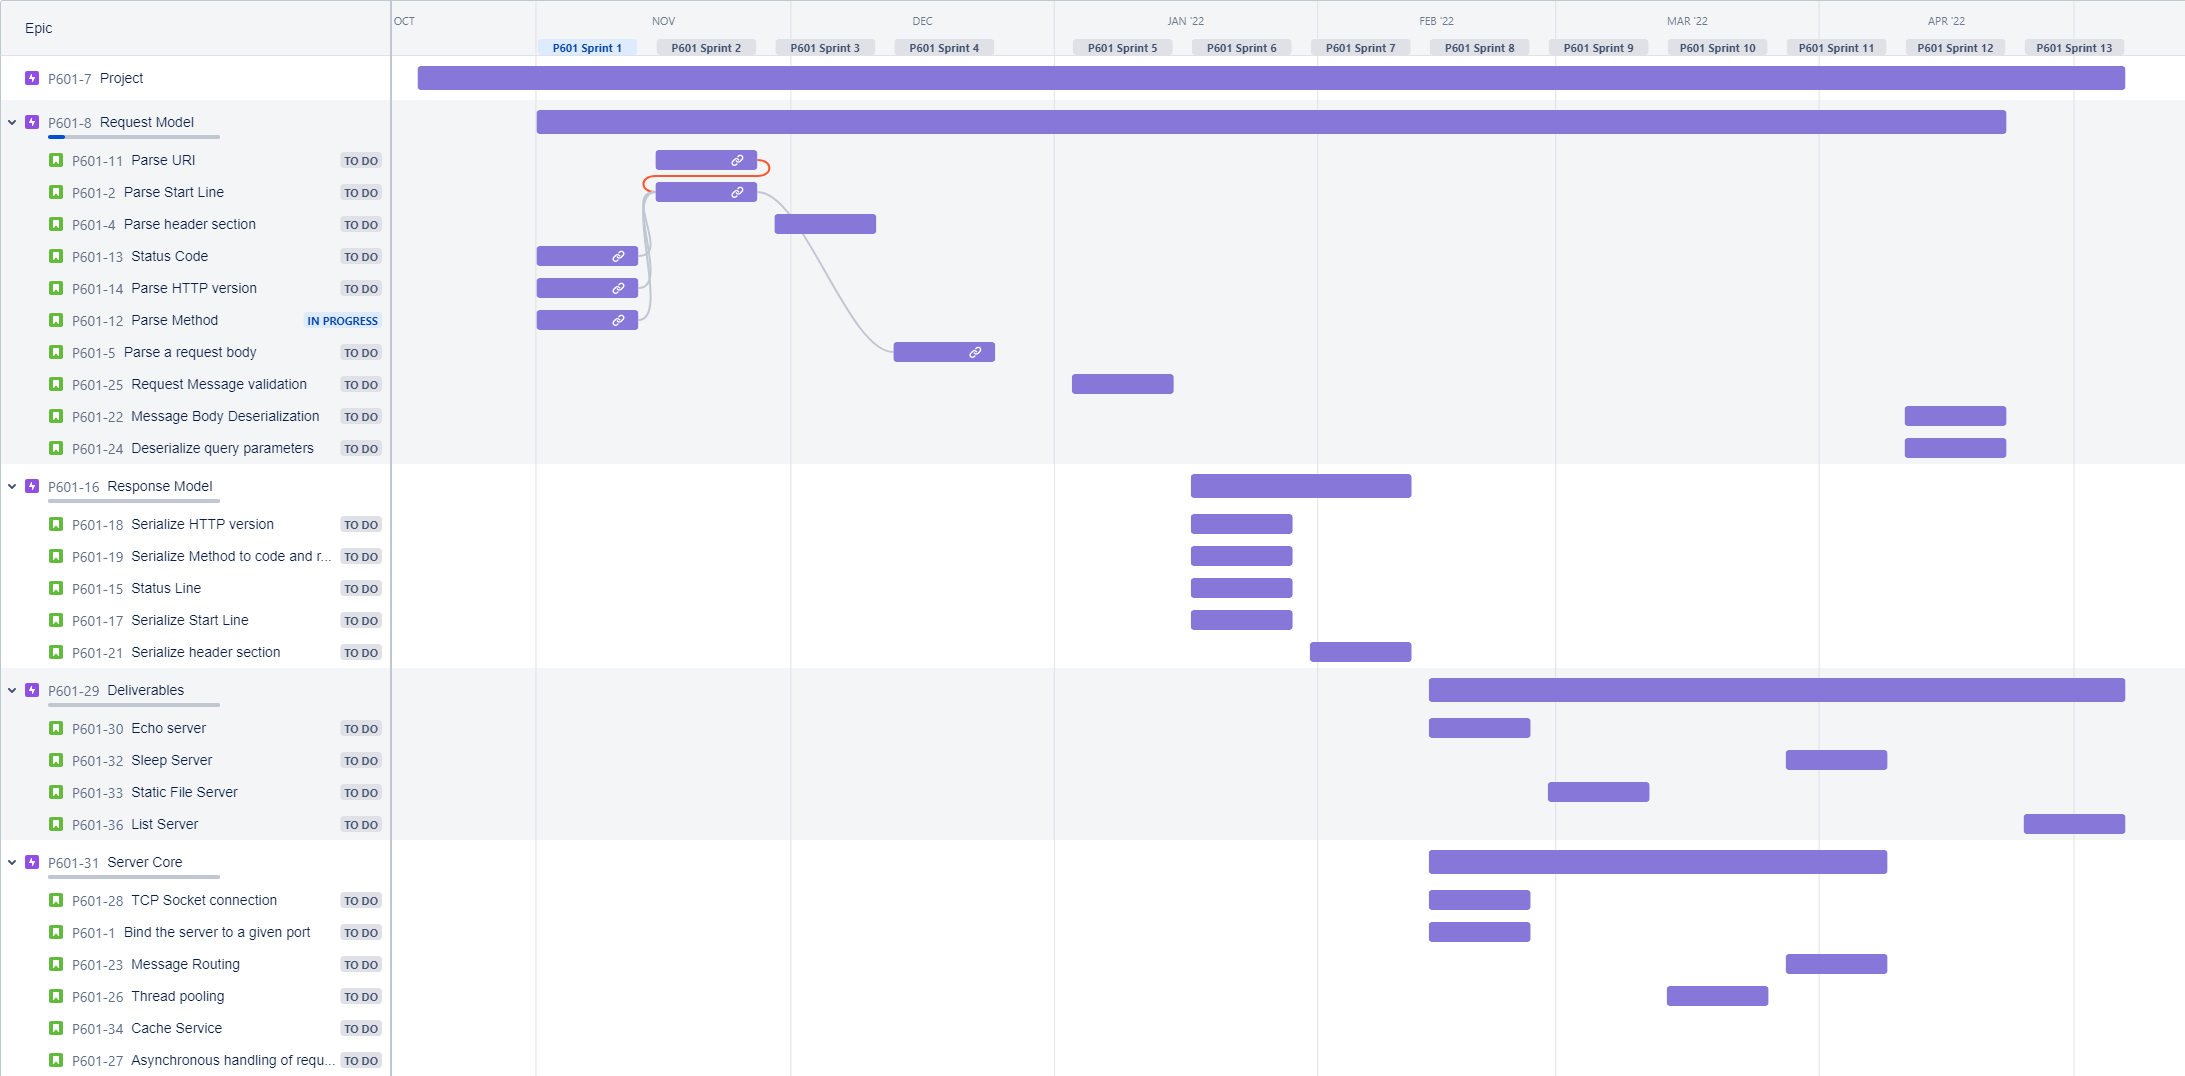
\includegraphics[width=1\textwidth]{project-roadmap.png}
  \caption{Jira roadmap}
  \label{fig:jira-roadmap}
\end{figure}

\subsection{Current Progress} \label{ss:current-progress}

As of this report the majority of the planning for the project has been completed and the end of
the first sprint coincides with the completion of this report. 

The planning is done in Jira and sprints have been scheduled, however, the detail of user stories and the
estimates of user stories further in the future are more conservative to account for the
\emph{Cone Of Uncertainty} (\cite{cone-of-uncertainty}). This allows me to follow the major requirements
of the plan and give me freedom to break the user stories into more fine-grained stories as the
level of uncertainty decreases over the development of the project.

The first sprint is on schedule to be completed successfully and included some project setup time
and completing of this interim report. On completing the sprint I will review the burndown chart
and the work completed and check if the next sprint has the correct amount of work given the current
early velocity of work. I will likely determine that more than one or two sprints will be required
to determine the velocity of my work which I can then apply to the remaining sprints.

\subsection{Risk Analysis}

A major concern is that the request parsing is so important to the rest of the library that an implementation
mistake or misguided API design could be discovered later in the project and would need to be resolved.
In part this is why the request and response are different epics even though there is a fair amount 
of overlap in data structures used. As explained in \textbf{\nameref{ss:current-progress}} I also
took into account the \emph{Cone of Uncertainty} by providing more conservative estimates for stories
further in the future.

The example deliverables are scope based and so this allows me to provide a deliverable to demonstrate
a set of features implemented. I had initially planned to implement the examples at the end of the
project, however, if I was unable to continue or the plan was running late then it could result in
the examples not being completed. In order to mitigate this I have planned to implement the examples
as soon as they can be supported by the library, this also allows me to review the library as a consumer
rather than a developer at an early stage in the project which might result in finding a bug or
ergonomic issues that would be easier to resolve earlier.

All the code and planning is stored in services external to my personal devices this mitigates any
local device malfunctions to only causing small loses in work.

\section{Additional Research}

This section reviews the additional research conducted which has not been cited above in this report.

Early research into using Rust for this project included reading multiple blogs
(\cite{knoldus-concurrency-in-rust}; \cite{ghostcell}; \cite{dblp-perfomance-vs-effort-rust-c}) including
what is known as \emph{The book}(\cite{rust-the-book}) and a white paper on how Rust was used in
NPM (\cite{rust-npm-paper}). This research included basics and advanced aspects of Rust and allowed
me to get a feel for the benefits of using Rust as explained in \nameref{ssec:language-and-dev-tools}.

When researching the parsing requirements for URIs used in the requests, I needed to review the
textual representation of Ipv4 and Ipv6 (\cite{rfc5952}), however, I won't need to
implement this parsing as the Rust language provides an implementation and an abstraction over both
respectively.

\newpage
\printbibliography

\end{document}
